%%%%%%%%%%%%%%%%%%%%%%%%%%%%%%%%%%%%%%%%%%%%%%%%%%%%%%%%%%%%%%%%%%%%
%% I, the copyright holder of this work, release this of into the
%% public domain. This applies worldwide. In some countries this may
%% not be legally possible; if so: I grant anyone the right to use
%% this work for any purpose, without any conditions, unless such
%% conditions are required by law.
%%%%%%%%%%%%%%%%%%%%%%%%%%%%%%%%%%%%%%%%%%%%%%%%%%%%%%%%%%%%%%%%%%%%

\documentclass[
    %twoside,   % Printed version
    %printed,   % Printed version
    digital,    % PC version
    oneside,    % PC version
    color,
    11pt,
    nocover,
    notable,
    nolof,
    nolot,
    final
  %% More options are listed in the user guide at
  %% <http://mirrors.ctan.org/macros/latex/contrib/fithesis/guide/mu/fi.pdf>.
]{fithesis3}
%% The following section sets up the locales used in the thesis.
\usepackage[resetfonts]{cmap} %% We need to load the a T2A font encoding
%\usepackage[utf8]{inputenc}
\usepackage[T1]{fontenc}  % T2a commented %% to use the Cyrillic fonts with Russian texts.
\usepackage[
  main=english, %% By using `czech` or `slovak` as the main locale
                %% instead of `english`, you can typeset the thesis
                %% in either Czech or Slovak, respectively.
  english, czech %german, russian, slovak %% The additional keys allow
]{babel}        %% foreign texts to be typeset as follows:
%%
%%   \begin{otherlanguage}{german}  ... \end{otherlanguage}
%%   \begin{otherlanguage}{russian} ... \end{otherlanguage}
%%   \begin{otherlanguage}{czech}   ... \end{otherlanguage}
%%   \begin{otherlanguage}{slovak}  ... \end{otherlanguage}
%%
%% For non-Latin scripts, it may be necessary to load additional
%% fonts:
%\usepackage{paratype}
%\def\textrussian#1{{\usefont{T2A}{PTSerif-TLF}{m}{rm}#1}}

%%
%% The following section sets up the metadata of the thesis.
\thesissetup{
    date          = \the\year/\the\month/\the\day,
    university    = mu,
    faculty       = fi,
    type          = mgr,
    author        = Michal Hajas,
    gender        = m,
    advisor       = {RNDr. Petr Švenda, Ph.D.},
    title         = {Statistical testing of lighweight cryptography based pseudo-random number generators},
    TeXtitle      = {Statistical testing of lighweight cryptography based pseudo-random number generators},
    keywords      = {randomness testing, cryptanalysis, block functions, lightweight cryptography, pseudo-radnom number generators},
    TeXkeywords   = {randomness testing, cryptanalysis, block functions, lightweight cryptography, pseudo-radnom number generators},
}


\thesislong{abstract}{%
Abstract to be done
}

\thesislong{thanks}{%
Thank all.


\vspace*{11cm}\noindent{}\hspace*{-0.1cm}
Computational resources were supplied by the Ministry of Education, Youth and Sports of the Czech Republic under the Projects CESNET (Project No. LM2015042) and CERIT-Scientific Cloud (Project No. LM2015085) provided within the program Projects of Large Research, Development and Innovations Infrastructures.\\\\%
%
We also acknowledge the support of Czech Science Foundation, the project GA16-08565S.
}

%% The following section sets up the bibliography.
\usepackage{csquotes}
\usepackage[              %% When typesetting the bibliography, the
  backend=biber,          %% `numeric` style will be used for the
  style=numeric,          %% entries and the `numeric-comp` style
  citestyle=numeric-comp, %% for the references to the entries. The
  sorting=none,           %% entries will be sorted in cite order.
  sortlocale=auto         %% For more unformation about the available
]{biblatex}               %% `style`s and `citestyles`, see:
%% <http://mirrors.ctan.org/macros/latex/contrib/biblatex/doc/biblatex.pdf>.
\addbibresource{thesis.bib} %% The bibliograpic database within
                          %% the file `example.bib` will be used.
\usepackage{makeidx}      %% The `makeidx` package contains
\makeindex                %% helper commands for index typesetting.



%% These additional packages are used within the document:
\usepackage{paralist}
\usepackage{amsmath}
\usepackage{amsthm}
\usepackage{amsfonts}
\usepackage{url}
\usepackage{menukeys}

% cref, has to be loaded after hyperref
\usepackage{hyperref}
\usepackage[noabbrev,capitalise]{cleveref}
% for long equation wrap
\usepackage{wrapfig}
% figure captions
\usepackage{caption}
% subcaption for 2 figures in one
\usepackage{subcaption}
% H figures
\usepackage{float}

% tables
\usepackage{tabularx}
% colored cells (cellcolor)
\usepackage{colortbl}

% my colours
\usepackage{xcolor}

%% My own inputs:
% enabling new fonts support (nicer)
\usepackage{lmodern}
% better typeset of line ends and so (nicer)
\usepackage{microtype}

\thesisload{}

\usepackage{tikz}
\usetikzlibrary{shapes,arrows,positioning}
\usetikzlibrary{decorations.pathreplacing}

% package to make bullet list nicer
\usepackage{enumitem}
\setitemize{noitemsep,topsep=3pt,parsep=3pt,partopsep=3pt}

% intendation
\usepackage{parskip}

% table colours
\newcommand{\fd}{\cellcolor{red!25}}
\newcommand{\fn}{}

% make captions italic
\usepackage[format=plain,
            font=it]{caption}

% Lubo's hack for margins
	\newcommand{\lmar}{3cm} % PC
	\newcommand{\rmar}{3cm} % PC
	\newcommand{\tmp}{3cm}  % PC

	%\newcommand{\lmar}{3.5cm} % Printed
	%\newcommand{\rmar}{2.5cm} % Printed
	%\newcommand{\tmp}{2.5cm}  % Printed


\usepackage[top=3cm, bottom=3.5cm, left=\lmar, right=\rmar]{geometry}

% Eliminates margins
\def\nomar{\list{}{\rightmargin-\tmp \leftmargin-\tmp}\item[]}
\let\endnomar=\endlist

% rotate figures
\usepackage{rotating}

% Table rotations
\usepackage{booktabs} % http://ctan.org/pkg/booktabs
\usepackage{xparse}   % http://ctan.org/pkg/xparse
% Rotation: \rot[<angle>][<width>]{<stuff>}
\NewDocumentCommand{\rot}{O{45} O{1em} m}{\makebox[#2][l]{\rotatebox{#1}{#3}}}%

% Rotates table cell
\newcolumntype{R}[1]{>{\begin{turn}{90}\begin{minipage}{#1}}l%
<{\end{minipage}\end{turn}}%
}


\begin{document}

% English indentation, vertical, not horizontal
\setlength{\parskip}{5pt}
\setlength{\parindent}{0pt}

%% We will define several mathematical sectioning commands.
%\newtheorem{theorem}{Theorem}[section] %% The numbering of theorems
                               %% will be reset after each section.
%\newtheorem{lemma}[theorem]{Lemma}     %% The numbering of lemmas
%\newtheorem{corr}[theorem]{Corrolary}  %% and corrolaries will
                                %% share the counter with theorems.
%\theoremstyle{definition}
%\newtheorem{definition}{Definition}
%\theoremstyle{remark}
%\newtheorem*{remark}{Remark}

\chapter{Introduction}
\label{chap:introduction}


\chapter{Theory}

\chapter{Introduction of CryptoStreams tool}
\label{chap:cryptostreams}

CryptoStreams tool is written in C++ language and is developed and maintained by team of people\footnote{The team of randomness testing involves following people: Radka Cieslarová, Michal Hajas, Dušan Klinec, Matúš Nemec, Jiří Novotný, Ľubomír Obrátil, Marek Sýs, Petr Švenda, Martin Ukrop and others.} at the Centre for Research on Cryptography and Security, Masaryk University~\cite{CryptoStreams}. The tool is used to generate output data streams from parametrized cryptographic functions. Each stream is configurable with resulting size and with several configuration options per individual streams such as seed, plaintext or key type. 

\section{History}

Initial implementation of CryptoStreams project was part of tool EACirc~\cite{EACirc} which is a tool for automatic randomness testing based on genetic programming. At that moment it served only as an input to EACirc and was not possible to use it separately outside of this project. After some time we decided that CryptoStreams might be potentially interesting also as a separate tool. That is why EACirc-streams project was introduced in 2017 and then in 2018 EACirc sub-name was completely abandoned and project was renamed to nowadays name, CryptoStreams.

\section{Idea}

Main idea behind CryptoStreams is easy production of data from crypto-primitives which are somehow reduced in complexity, either by rounds or by providing them input with bad randomness properties. By analyzing such outputs, for example, with statistical batteries or other randomness testing tools, it is possible to discover potential weaknesses in investigated functions. In this thesis we will present usage of CryptoStreams for generation of streams followed by statistical testing using well known statistical batteries and Booltest~\cite{booltest-secrypt2017} on functions designed for internet of things, also called lightweight functions.

\section{Content of CryptoStreams}

In this section we would like to present deeper details about what this tool provides. Very first cryptoprimitives which were added to CryptoStreams were candidates from SHA-3 and eStream competitions. Those additions were done by Ondrej Dubovec~\cite{Dubovec2012thesis} and Matej Prišťák~\cite{Pristak2012thesis} in 2012. Within those theses were added 34 hash functions and 27 stream ciphers. Another addition was done by Martin Ukrop in his master thesis~\cite{Ukrop2016thesis} regarding authenticated encryption systems from CAESAR competition~\cite{caesar-competition}. CryptoStreams also contains well known block ciphers like AES, DES etc. Block ciphers were added by Karel Kubíček~\cite{Kubicek2017thesis} and Tamás Rózsa~\cite{Rozsa2018thesis} in their theses. There are also lot of other cryptoprimitives added outside of thesis or papers.

% TODO: find citations for SHA-3 and eStream competition

Part of this thesis is also addition of pseudo-random number generators to project. This component is still in development and serves only as potential start point for future work. We added together 6 generators. 3 of them from standard library, namely \textit{\textbf{lcg}}~\footnote{\url{ https://en.cppreference.com/w/cpp/numeric/random/linear\_congruential\_engine}}, \textbf{\textit{mersenne twister}}~\footnote{\url{https://en.cppreference.com/w/cpp/numeric/random/mersenne\_twister\_engine}} and \textbf{\textit{substract with carry}}~\footnote{\url{https://en.cppreference.com/w/cpp/numeric/random/subtract\_with\_carry_engine}}. The other 3 are from TesU01~\cite{l2007testu01} project, namely \textbf{\textit{lcg}}, \textbf{\textit{mrg}} and \textbf{\textit{xorshift}}, more information in user guide~\cite{LEcuyer07testu01}. Pseudo random generators were added including some basic tests.

\subsection{Details of stream generation}

Each output is generated by so called \textit{streams} which are producers of data. Retrieving data from \textit{stream} in a loop and storing them results in data file with desired binary data. Each call for new data from stream will return data of adjustable size, so called \textit{test-vector size}. By setting size of test-vector and number of test vector it is possible to set size of resulting data file. CryptoStreams contains following types of streams.

\begin{description}
	\item[Streams based on round-reduced cryptoprimitives.] Besides the round limitation it is also possible to configure them with various types of plaintext and key inputs. For example, it is possible to obtain data from AES limited to 3 rounds which are generated by encrypting all zeroes plaintext with key consisting of all ones. 
	\item[Streams outputing data of exact structure] which are mostly used as an input streams such as plaintext or key stream. Those might be for example binary zero, binary one stream or low hamming weight stream (small amount of ones) etc. Random (pseudo-random) streams also belong to this category.
	\item[Manipulating streams] are configured with some source stream or more streams and manipulate them in some desired way. For example, repeating stream is repeating one output specified number of times before generating new test-vector. Another example is tuple stream that is getting more streams as an input and for each call it returns test-vector which contains data from each stream concatenated together. By tuple stream it is possible to receive data which consists of plaintexts followed by corresponding ciphertexts. 
\end{description}


\subsection{Configuration}

All necessary configuration within one run is achieved by \texttt{JSON} file. All possible options how to configure CryptoStreams can be found in project documentation~\cite{CryptoStreams-wiki}
JSON, test vectors (size/count), seeding

\subsection{Testing of streams (Google testse), testing with test vectors, functional tests}

\section{Test with statistical batteries/ RTT}

\section{Conducted experiments}

There are more ways how we reduce functions so that we find out where are theirs limitations. 

\begin{description}
	\item[Special type of input,] mostly with some bad randomness properties, is provided to functions and then results are compared with random or other special inputs. For puposes of this thesis we used following types of streams.
	\begin{enumerate}
		\item Counter stream is a stream in which each test-vector is addition of one to previous test-vector in number representation.
		\item Low hamming weight stream returns outputs with least count of ones it is possible. Starting with all zeroes. Then only binary one on each position etc.
		\item Strict avalanche criterion is a type of stream in which first test-vector is randomly generated and every next call is just previous test-vector with one flipped bit.
	\end{enumerate}


	\item[Round reduced] function, is such function, which is composed of very same sequence of operations performed multiple times, mostly in a loop. For example, AES~\cite{FIPS-197} has recommended number of rounds 10, 12 or 14 based on key length as you can see in \cref{fig:fips197-rounds}. Each round in AES consists of \textbf{\textit{SubBytes, ShiftRows, MixColumns, AddRoundKey}} operations.
	
	\begin{figure}[h]
		\centering
		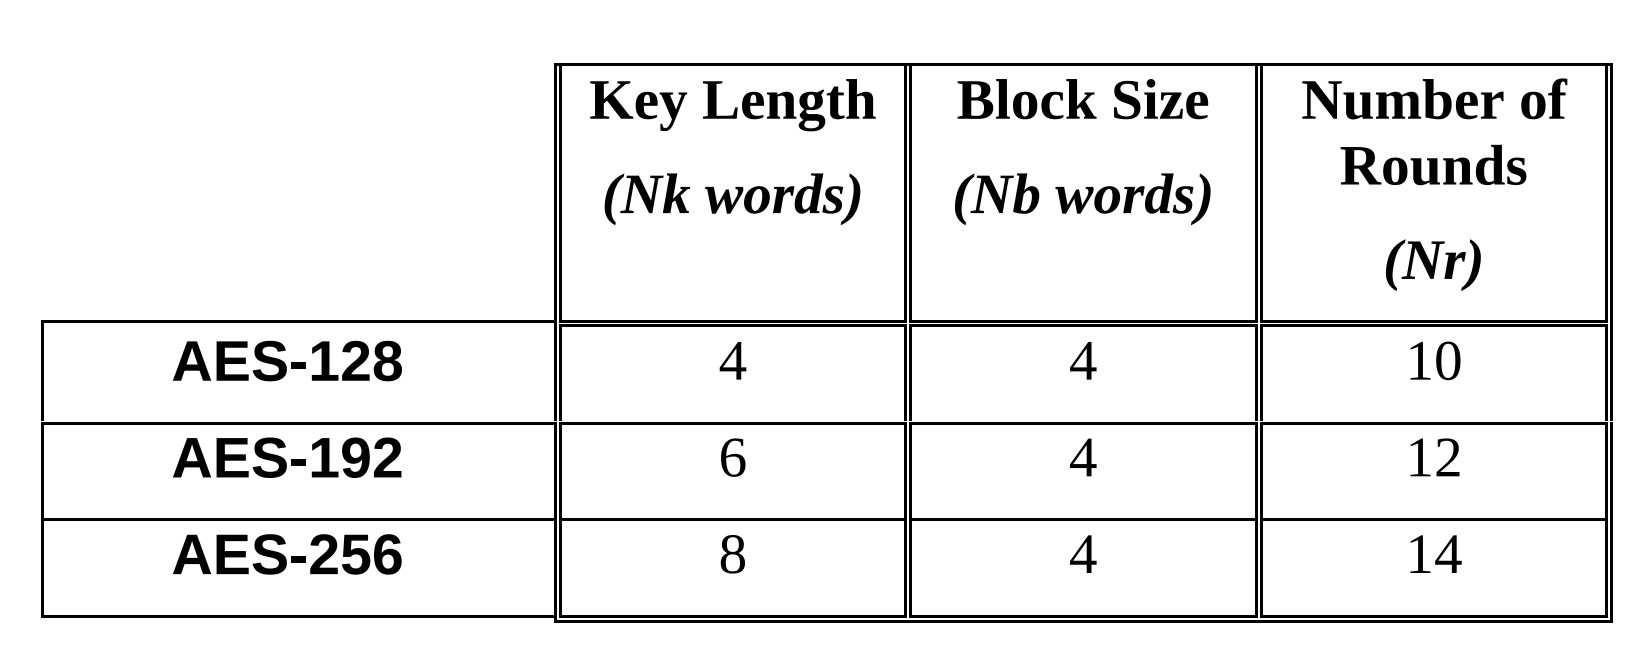
\includegraphics[width=0.9\textwidth]{./images/pictures/FIPS197-Nr-table.png}
		\caption{Table of rounds based on key size taken from~\cite{FIPS-197}, word size is 32 bits.}
		\label{fig:fips197-rounds}
	\end{figure}

	By analyzing differences between pseudo-randomness of individual rounds it is possible to find out so called \textbf{security margin}. Denoting security margin involves finding out how many rounds is breakable by any kind of attack, the less rounds we are able to break, the higher security margin is. In this thesis we will denote security margin by randomness properties of individual round output.
	
% TODO: Find out security margin literature
	\item[Plaintext ciphertext stream] produce pairs of input and output to function. With statistical testing performed on such output, it is possible to investigate dependency between plaintext and ciphertext. However we need to be careful with deciding what input we will choose since it is part of output it must have perfect randomness properties otherwise it may cause some interference in testing result.

\end{description}

\section{Investigated functions}

Source code of investigated functions were taken over from project FELICS~\cite{dinu2015felics} developed by Daniel Dinu and his group at University of Luxembourg. This project is conducting performance analysis of functions that are intended for internet of things devices. We have taken over only C++ implementation of functions, as we were not interested in implementations optimized for other architectures. Also we needed to implement round reduction of functions ourselves as the project contained only full round implementation. However, provision of round reduction was not hard, mostly functions were prepared with round reduction in mind and we needed to only replace constant in loop with our variable. 

Besides the main loop, functions mostly contain also key scheduling, initial and final part. Key scheduling is taking care of the creation of round key based on a encryption key. Initial and final part serves for initialization and finalization of process. We do not round-reduce any of those parts as we wanted to avoid some memory problems like uninitialized or wrongly cleaned memory.

\cref{table:list-of-investigated functions} contains all investigated functions including some basic information about them. Our intention was also adding two test scenarios for each added function. First scenario is testing correct implementation with test vectors. We used test vectors from FELICS project as it contains test vectors for each function. The aim of the second test scenario is testing round reduction by doing encryption followed by decryption and checking of correct decrypted plaintext. However, we were not able to make this scenario work for each function. Function without this test are marked with \textit{no} in last column in \cref{table:list-of-investigated functions}. The main reason why we were not able to make this test work is that FELICS project is not build to support it and we were not able to modify it in a way it would work. This may be caused also by non reducing of key scheduling, initial and final parts. However this is just an optional test and it is not crucial for functions to pass it. The most important is that the test is passing in full round version of function.
\begin{table}[t]
	\centering
	\begin{tabular}{c|c c c c}
		\textbf{\large Function} & \textbf{\large Round} & \textbf{\large Block size} & \textbf{\large Key size} & \textbf{\large Encrypt Decrypt test}\\ \hline
		Chaskey			& 16	& 16	& 16	& yes 	\\ \hline
		Fantomas		& 12	& 16	& 16	& yes 	\\ \hline
		HIGHT			& 32	& 8		& 16	& no 	\\ \hline
		LBlock			& 32	& 8		& 10	& no \\ \hline
		LEA				& 24	& 16	& 16	& no \\ \hline
		LED 			& 48	& 8		& 10	& yes \\ \hline
		Piccolo			& 25	& 8		& 10	& yes \\ \hline
		PRIDE			& 20	& 8		& 16	& no  \\ \hline
		PRINCE			& 12	& 8		& 16	& yes \\ \hline
		RC5-20			& 20	& 8		& 10	& yes \\ \hline
		RECTANGLE-K80	& 25	& 8		& 16	& no \\ \hline
		RECTANGLE-K128	& 25	& 8		& 16	& no \\ \hline
		RoadRunneR-K80	& 10	& 8		& 10	& yes \\ \hline
		RoadRunneR-K128	& 12	& 8		& 16	& yes \\ \hline
		Robin			& 16	& 16	& 16	& yes \\ \hline
		RobinStar		& 16	& 16	& 16	& yes \\ \hline
		SPARX-B64		& 8		& 8		& 16	& yes \\ \hline
		SPARX-B128		& 8		& 16	& 16	& yes \\ \hline
		TWINE			& 35	& 8		& 10	& yes \\ \hline
		
		
	\end{tabular}
	\caption{List of all investigated functions, where sizes are given in Bytes. Including information whether encrypt decrypt test passed.}
	\label{table:list-of-investigated functions}
\end{table}



\chapter{Results of evaluation of statistical randomness properties}


%%bibliography

\printbibliography[heading=bibintoc] %% Print the bibliography.

\appendix{}

\end{document}
